\section{Theorie}
\label{sec:Theorie}

\subsection{Klassische Physik vs. Quantenmechanik}
Die Ausbreitung des Lichts unterliegt den Gesetzen der geometrischen Optik und kann makroskopisch sehr genau vorhergesagt werden.
Schattenwurf, Streuung/Spiegelung an festen Objekten oder die Brechung des Lichts an Linsen oder Prismen unterliegen einfachen geometrischen Beziehungen, wie etwa der \textit{Linsengleichung}\cite[286]{taschenbuch}.
Es gibt jedoch Bedingungen, bei denen diese Modelle nicht mehr angewendet werden können.
Diese Abweichungen treten unter anderem dann auf, wenn Licht auf Hindernisse trifft und der Strahldurchmesser größer als das Hindernis selbst ist.
Sie treten auch dann auf, wenn das Licht auf Spalte in Schirmen trifft.\\
Es kann jedoch über eine große Anzahl von Lichtquanten gemittelt und die Phänomene über das klassische Wellenmodell erklärt werden.
Dieser Ansatz wird hier genutzt.\\

\subsection{Beugung am Spalt}
Grundlage für die Beugung des Lichts ist das \textit{Huygens-Prinzip}.
Nach diesem Prinzip ist jeder Punkt einer Wellenfront stets Erzeugungspunkt neuer Kugelwellen, den sogenannten \textit{Elementarwellen}.
Bei einem langen, schmalen Spalt entstehen durch diese Eigenschaft Zylinderwellen entlang der Spaltebene.


\begin{figure}
    \centering
    \begin{subfigure}{.5\textwidth}
      \centering
      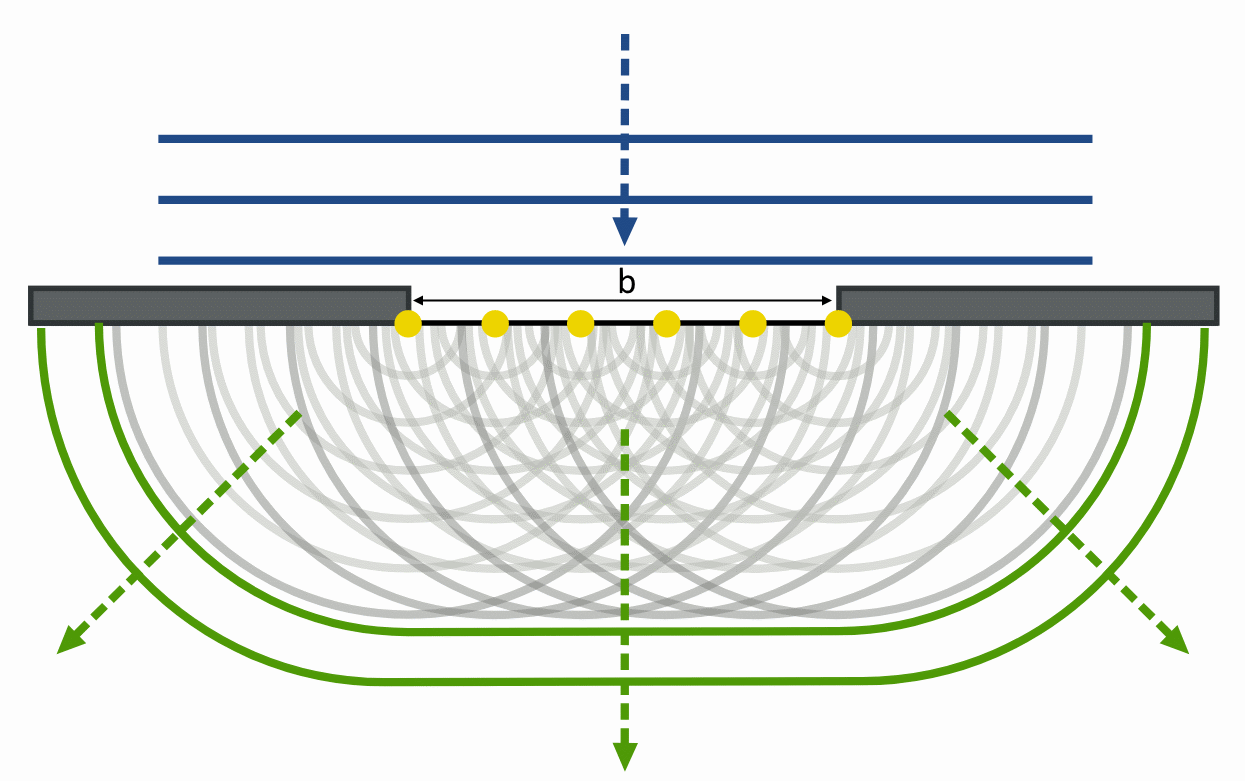
\includegraphics[width=.45\textwidth]{plots/Huygens.png}
    \caption{Überlagerung von Kugelwellen an einem Einzelspalt.\cite{HuygensWiki}}
    \label{fig:huygens}
    \end{subfigure}%
    \begin{subfigure}{.5\textwidth}
      \centering
      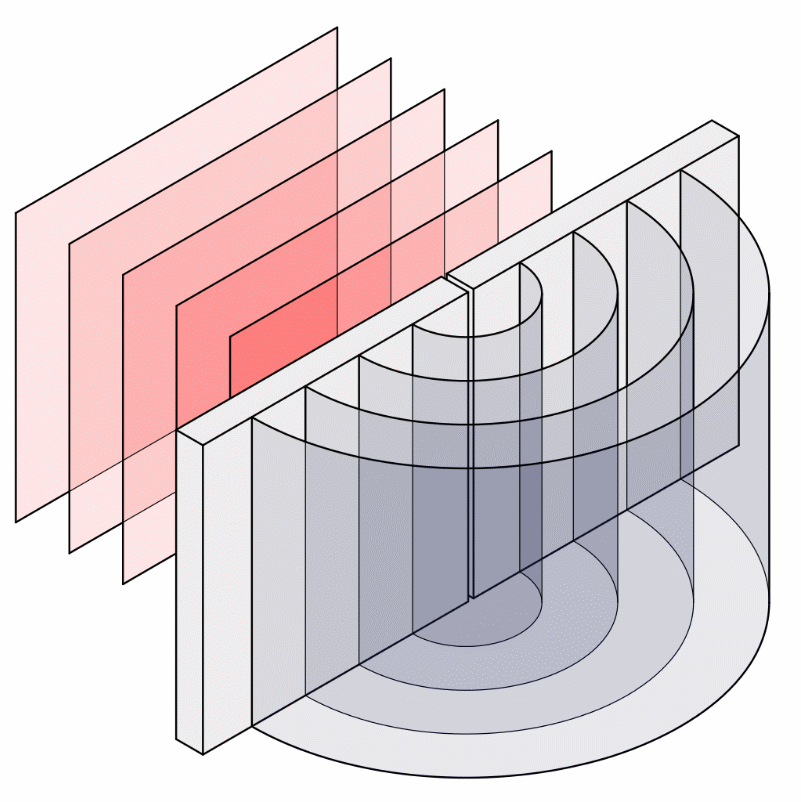
\includegraphics[width=.45\linewidth]{plots/Zylinderwellen.png}
      \caption{Zylinderwellen am Einzelspalt.\cite{BeugungWiki}}
      \label{fig:zylinder}
    \end{subfigure}
    \label{fig:huygenZylinder}
\end{figure}

\subsection{Einzelspalt}
Die am Spalt entstehenden Zylinderwellen überlagern sich und interferieren miteinander. Das daraus entstehende Abbild, die \textit{Beugungsfigur}, ist eine Amplituden-Funktion $B(\varphi, \lambda, b, d)$ des Abstrahlwinkels $\varphi$,
der Wellenlänge $\lambda$, der Spaltbreite $b$ und des Abstandes $d$ zum Beobachtungspunkt.
In diesem Versuch wird die Funktion in Abhängigkeit des Abstrahlwinkels untersucht, sodass die anderen Parameter konstant bleiben.
Gesucht ist also die Funktion $B(\varphi)$.

\subsubsection{Einschub: Nahfeld und Fernfeld}
Geometrisch bedingt weist eine Beugungsfigur in einem Nahfeld nur wenig Interferenz auf und ist für diesen Versuch nicht von Interesse.
Damit zwei Wellen interferieren, muss die Richtung des Wellenvektors $\vec{k}$ parallel, oder in etwa gleich sein. Im Falle der Zylinderwellen reduziert sich % Literatur wäre schön
die Bedingung an die Raumrichtung auf nur eine Dimension, und damit auf den Abstrahlwinkel $\varphi$.
Da die Winkelunterschiede in einem Nahfeld zu groß werden, entsteht keine oder nur wenig Interferenz.

\begin{figure}
    \centering
    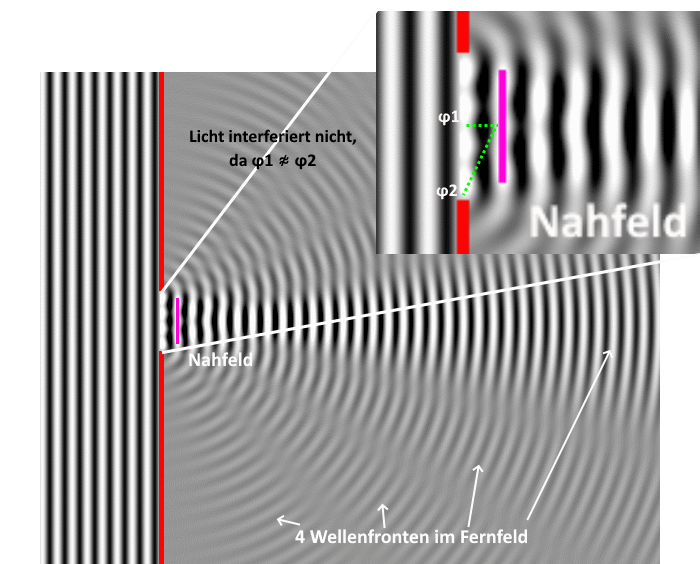
\includegraphics[width=0.9\textwidth]{plots/Wave_Diffraction_4Lambda_Slit.png}
    \caption{Beugung ebener Welle am Einzelspalt mit $b = 4\lambda$.\protect\footnotemark\:\cite{OptischerspaltWiki}}        % Kommentar für selbst: Sehr nützlich, um Fußnoten in Bildunterschriften hinzuzufügen. Das protect sorgt dafür, dass die Fußnote auf derselben Seite erscheint.
    \label{fig:waveDiff}
\end{figure}
\footnotetext{$b\:\hat{=} $ Spaltbreite und $\lambda\:\hat{=} $ Wellenlänge der ebenen Wellen.}

Dieser Grenzfall kann ausgeschlossen werden, indem der Abstand zwischen Spalt und Schirm hinreichend groß gewählt wird (s. Abb. \ref{fig:fresnelFraunhofer}).
In diesem Fall wird eine Sammellinse verwendet, um die von der Spaltöffnung ausgehenden, parallelen Lichtstrahlen mit gleichem Abstrahlwinkel auf einen Beobachtungspunkt $P$ zu fokussieren. Die Lichtfront kommt hierbei aus dem Unendlichen. Dieser Fall wird \textit{Fraunhofer-Beugung} genannt.
Falls keine Sammellinse verwendet wird, liegen Lichtquelle und Beobachtungspunkt $P$ im Endlichen und es gilt $b \ll d : \varphi_1 \approx \varphi_2$.\:\footnote{$d\:\hat{=} $Abstand Spalt-Beobachtungspunkt.} Dieser Fall heißt \textit{Fresnel-Beugung} (s. Abb. \ref{fig:fresnelFraunhofer}).

\begin{figure}
    \centering
    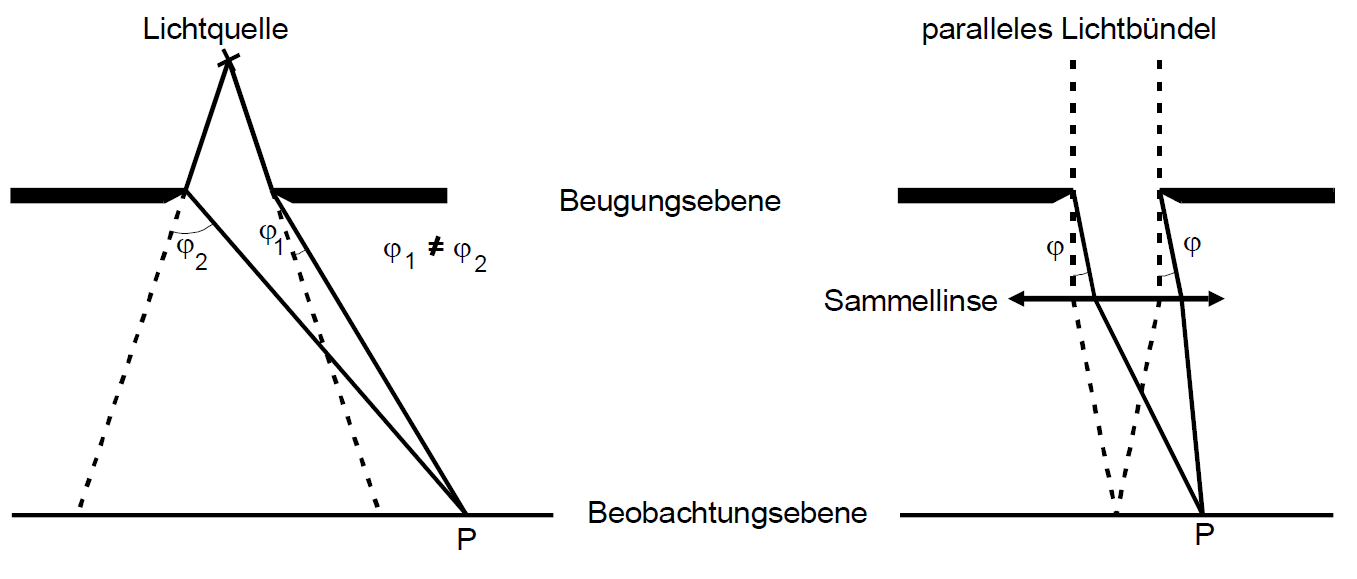
\includegraphics[width=0.8\textwidth]{plots/Fresnel_Fraunhofer.png}
    \caption{Fresnel- (links) und Fraunhofer-Beugung (rechts) an einem Einzelspalt.\protect\footnotemark}
    \label{fig:fresnelFraunhofer}
\end{figure}

\subsection{Amplituden-Funktion}
Der Phasenunterschied $\delta$ zweier paralleler Lichtstrahlen steht in geometrischer Beziehung zum Entstehungspunkt auf der Spaltebene (s. Abb. \ref{fig:BeugSpalt}).
Die absolute Länge $s$ der Phasendifferenz zu einem gleichzeitig entstehenden Lichtstrahl mit Abstand $x$ ist mit einem Abstrahlwinkel von $\varphi$
\footnotetext{Abbildung angelehnt an Versuchsanleitung.\cite{Versuchsanleitung}}

\begin{equation}
  s = x\sin{\varphi} \:.
  \label{eqn:s}
\end{equation}

\begin{figure}
  \centering
  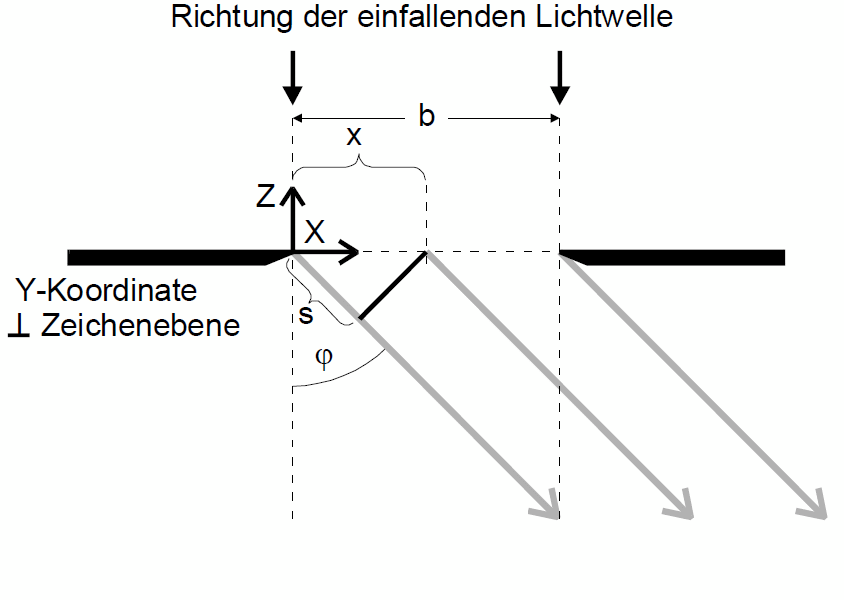
\includegraphics[width=0.8\textwidth]{plots/Beugung Einzelspalt.png}
  \caption{Geometrische Betrachtung der Beugung am Spalt.\cite{Versuchsanleitung}}
  \label{fig:BeugSpalt}
\end{figure}

Daraus folgt die Phasendifferenz

\begin{equation}
  \delta = \frac{s}{\lambda}2\pi \:.
  \label{eqn:delta}
\end{equation}



Eine ebene Welle besitzt die Amplituden-Funktion 
\begin{equation}
  A(z, t) = A_0e^{i(\omega t - kz)} \:.
\end{equation}

Eine zusätzliche Phasendifferenz drückt sich in einer Addition des Exponenten aus.
\begin{equation*}
  A(z, t) = A_0e^{i(\omega t - kz + \delta)}
\end{equation*}

Um die überlagerte Amplitude unter Berücksichtigung der Phasendifferenz zu erhalten, wird über die gesamte Spaltbreite $b$ integriert.
Die Abhängigkeit des Phasenunterschiedes von $\varphi$ liefert somit eine indirekte Ortsangabe des Beobachtungspunktes.
Es wird über infinitesimale Abstände $dx$ der Lichtstrahlen integriert.

\begin{equation}
  B(z, t, \varphi) = A_0\int_0^be^{i(\omega t - kz + \delta(\varphi))}dx
  \label{eqn:B1}
\end{equation}

Nach einsetzen von \eqref{eqn:s} in \eqref{eqn:delta} und \eqref{eqn:delta} in \eqref{eqn:B1} folgt
\begin{equation*}
  B(z, t, \varphi) = A_0e^{i(\omega t - kz)}\int_0^be^{\frac{i2\pi x \sin{\varphi}}{\lambda}}dx \:.
\end{equation*}

Lösen des Integrals führt zu
\begin{equation}
  B(z, t, \varphi) = A_0\frac{\lambda}{i2\pi \sin{\varphi}}e^{i(\omega t - kz)}(e^{\frac{i2\pi b \sin{\varphi}}{\lambda}}-1) \:.
  \label{eqn:nachInt}
\end{equation}

Als Hilfestellung wird die eulersche Formel für den Sinus verwendet.
\begin{equation}
  \sin{\varphi} = \frac{1}{2i}(e^{i\varphi}-e^{-i\varphi})
  \label{eqn:eulerSin}
\end{equation}

Ausklammern in Gl. \eqref{eqn:nachInt} ergibt
\begin{equation}
  B(z, t, \varphi) = A_0\frac{\lambda}{\pi \sin{\varphi}}e^{i(\omega t - kz)}e^{\frac{i\pi b \sin{\varphi}}{\lambda}}\frac{1}{2i}(e^{\frac{i\pi b \sin{\varphi}}{\lambda}}-e^{-\frac{i\pi b \sin{\varphi}}{\lambda}}) \:.
  \label{eqn:ausgeklammert}
\end{equation}

Wird nun die eulersche Formel aus \eqref{eqn:eulerSin} in \eqref{eqn:ausgeklammert} angewendet, reduziert sich die Funktion zu
\begin{equation}
  B(z, t, \varphi) = A_0\frac{\lambda}{\pi \sin{\varphi}}e^{i(\omega t - kz)}e^{\frac{i\pi b \sin{\varphi}}{\lambda}}\sin{\frac{\pi b \sin{\varphi}}{\lambda}} \:.
  \label{eqn:ampLang}
\end{equation}

Der Faktor $e^{i(\omega t - kz)}$ ist der orts- und zeitabhängige Amplitudenkoeffizient und kann experimentell nicht berücksichtigt werden. Stattdessen wird mit $A_0$ gemittelt
und der Term reduziert.
Der zweite Term $e^{\frac{i\pi b \sin{\varphi}}{\lambda}}$ stellt einen Phasenfaktor dar und fällt wegen der Mittelung über alle Lichtquanten ebenfalls weg.
Wird ein zusammenfassender Ausdruck $\gamma := \frac{\pi b \sin{\varphi}}{\lambda}$ in \eqref{eqn:ampLang} eingesetzt, vereinfacht sich die Amplituden-Funktion mit einer alleinigen Abhängigkeit von $\varphi$ zu

\begin{equation}
  B(\varphi) = A_0b\frac{\sin{\gamma}}{\gamma}
\end{equation}
mit $\gamma := \gamma(\varphi)$.

Gemessen wird die nicht-negative Lichtintensität $I(\varphi)$, welche näherungsweise quadratisch mit der Amplitude wächst.
\begin{equation}
  I(\varphi) \propto B(\varphi)^2 = A_0^2b^2\frac{\sin^2{\gamma}}{\gamma^2}
  \label{eqn:I}
\end{equation}

\subsection{Doppelspalt}
Die Beugungsfigur des Doppelspalts ist eine multiplikative Überlagerung der beiden Einzelspalte.
Die Intensitätsverteilung der Figur ist gegeben durch eine zusätzliche Cosinus-Verteilung\cite{Versuchsanleitung}
\begin{equation}
  I(\varphi) \propto B(\varphi)^2 = 4A_0^2cos^2{(\frac{\gamma s}{b})}\frac{\sin^2{\gamma}}{\gamma^2}
  \label{eqn:doppelspalt}
\end{equation}
mit der zusätzlichen Größe $s$ als Abstand der beiden Spalte.

\begin{figure}
  \centering
  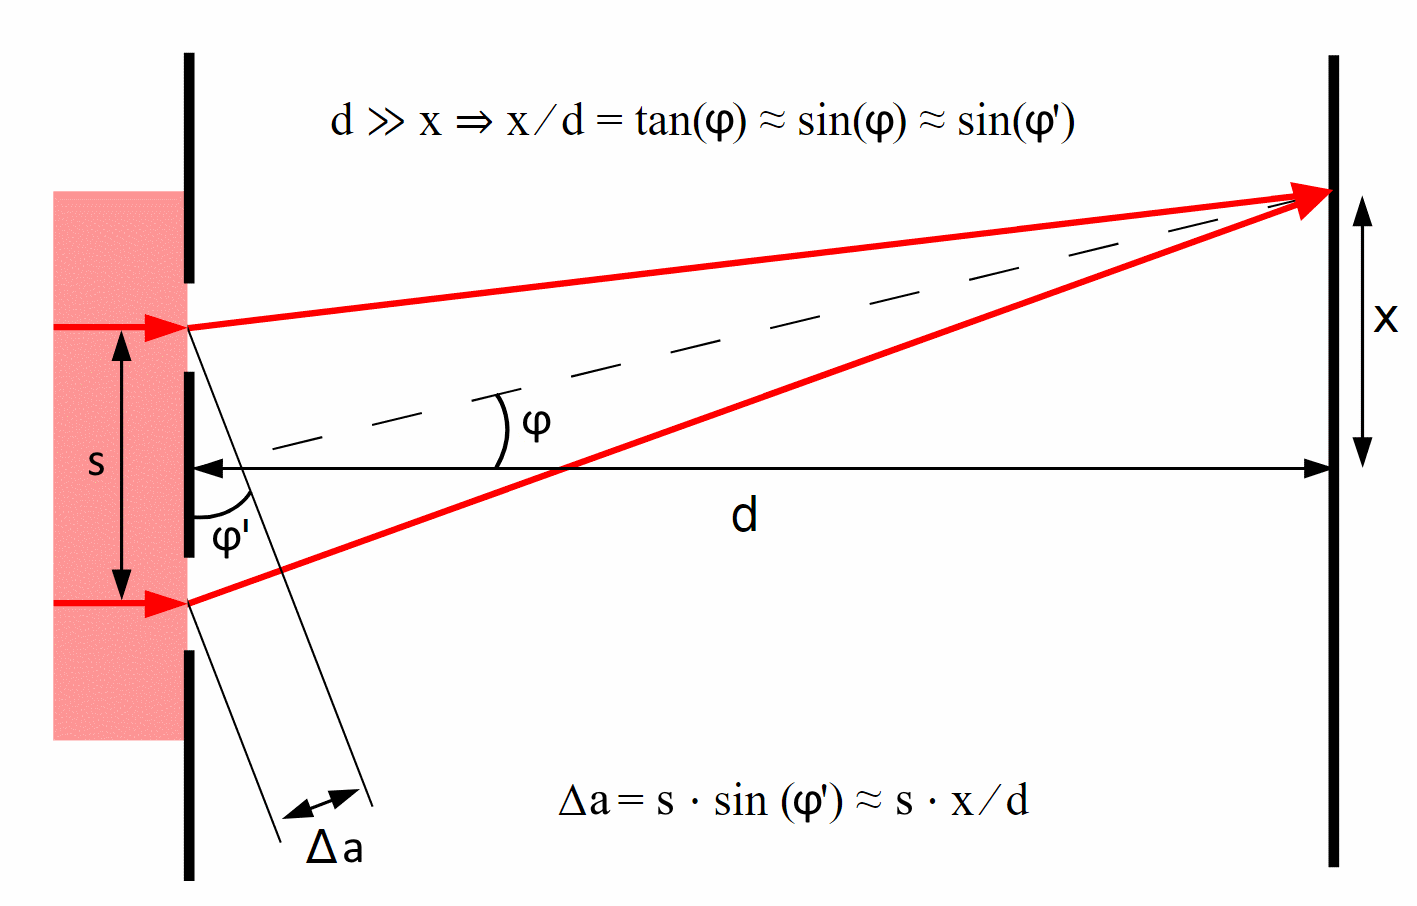
\includegraphics[width=.9\textwidth]{plots/Doppelspalt.png}
  \caption{Schematische Darstellung eines Doppelspalts.\cite{DoppelspaltWiki}}
  \label{fig:schemDoppel}
\end{figure}

\subsection{Fouriertransformation}
Die Amplituden-Funktion $B(\varphi)$ kann als Fourier-Transformierte aufgefasst werden.
Wird nun der Ansatz
\begin{equation}
  B(\eta) = \int_{0}^{b}A_0e^{ix\eta}
\end{equation}
gelöst, ergibt sich
\begin{equation}
  B(\eta) = \frac{2A_0}{\eta}e^{\frac{i\eta b}{2}}\sin{\frac{2\eta}{b}} \:.
\end{equation}
Wird der Realteil separiert und $\eta := \dfrac{2\pi \sin{\varphi}}{b}$ gewählt, ist das Ergebnis die ursprüngliche Funktion aus \eqref{eqn:doppelspalt}.
\begin{equation}
  Re(e^{\frac{i\eta b}{2}}) = \cos{\frac{\eta b}{2}}
\end{equation}
\begin{equation}
  B(\eta) = 2A_0b\:\cos{(\frac{\eta b}{2})}\:\:\frac{\sin{\frac{2\eta}{b}}}{\frac{2\eta}{b}}
  \label{eqn:fastDoppel}
\end{equation}
Die Gleichung \eqref{eqn:fastDoppel} kann nun mit $\gamma = \frac{2\eta}{b}$ in \eqref{eqn:doppelspalt} überführt werden.

\subsection{Umrechnung der Abstandsmessung zum Abstrahlwinkel}
Gemessen wird die absolute Position $x$ des Sensors mit unbekanntem Winkel $\varphi$ zur optischen Achse.
Der Winkel wird indirekt über den Abstand des Photoelementes zum Intensitätsmaximum $x_0$ bestimmt.
Das Maximum wird hierbei aus den Messdaten ermittelt.

\begin{equation}
  \sin{\varphi} = \frac{x'}{d'} = \frac{x'}{\sqrt{d^2+x'^2}}
\end{equation}
\begin{equation}
  x' = |x-x_0|
\end{equation}

\begin{figure}
  \centering
  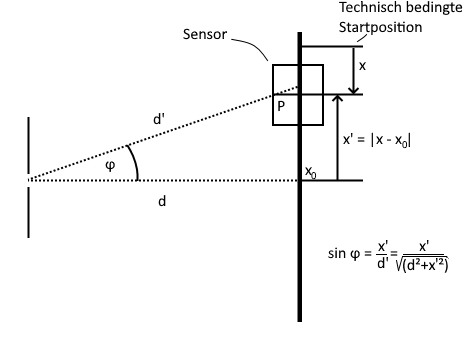
\includegraphics[width=.8\textwidth]{plots/x_to_angle.png}
  \caption{Relation zwischen Winkel $\varphi$ und Messgröße $x$.}
  \label{fig:xToAngle}
\end{figure}